%; whizzy paragraph -pdf xpdf -latex ./whizzypdfptex.sh
%; whizzy-paragraph "^\\\\begin{frame}\\|\\\\emtext"
% latex beamer presentation.
% platex, latex-beamer でコンパイルすることを想定。 

%     Tokyo Debian Meeting resources
%     Copyright (C) 2012 Junichi Uekawa
%     Copyright (C) 2016 Nobuhiro Iwamatsu

%     This program is free software; you can redistribute it and/or modify
%     it under the terms of the GNU General Public License as published by
%     the Free Software Foundation; either version 2 of the License, or
%     (at your option) any later version.

%     This program is distributed in the hope that it will be useful,
%     but WITHOUT ANY WARRANTY; without even the implied warreanty of
%     MERCHANTABILITY or FITNESS FOR A PARTICULAR PURPOSE.  See the
%     GNU General Public License for more details.

%     You should have received a copy of the GNU General Public License
%     along with this program; if not, write to the Free Software
%     Foundation, Inc., 51 Franklin St, Fifth Floor, Boston, MA  02110-1301 USA

\documentclass[cjk,dvipdfmx,12pt]{beamer}
\usetheme{Tokyo}
\usepackage{monthlypresentation}

%  preview (shell-command (concat "evince " (replace-regexp-in-string "tex$" "pdf"(buffer-file-name)) "&")) 
%  presentation (shell-command (concat "xpdf -fullscreen " (replace-regexp-in-string "tex$" "pdf"(buffer-file-name)) "&"))
%  presentation (shell-command (concat "evince " (replace-regexp-in-string "tex$" "pdf"(buffer-file-name)) "&"))

%http://www.naney.org/diki/dk/hyperref.html
%日本語EUC系環境の時
\AtBeginDvi{\special{pdf:tounicode EUC-UCS2}}
%シフトJIS系環境の時
%\AtBeginDvi{\special{pdf:tounicode 90ms-RKSJ-UCS2}}

\newenvironment{commandlinesmall}%
{\VerbatimEnvironment
  \begin{Sbox}\begin{minipage}{1.0\hsize}\begin{fontsize}{8}{8} \begin{BVerbatim}}%
{\end{BVerbatim}\end{fontsize}\end{minipage}\end{Sbox}
  \setlength{\fboxsep}{8pt}
% start on a new paragraph

\vspace{6pt}% skip before
\fcolorbox{dancerdarkblue}{dancerlightblue}{\TheSbox}

\vspace{6pt}% skip after
}
%end of commandlinesmall

\title{Debian Update}
\subtitle{OSC 2023 Online/Spring \\東京エリアDebian勉強会(出張版)}
\author{Debian JP Project \\杉本 典充\\ dictoss@debian.or.jp}
\date{2023-03-11}
\logo{
\includegraphics[width=8cm]{image-assets/openlogo-light.eps}}

\begin{document}

%-------------------

\section{表紙}

\begin{frame}
\titlepage{}
\end{frame}

\section{目次}

\begin{frame}{Agenda}
  \begin{itemize}
  \item Debian とは?
  \item Debian JP Project と Debian 勉強会
  \item 次期安定版 Debian 12 bookworm
    % \item Debian Updates
  \item 日本語における Debian の情報
  \item 今後のイベント
  \end{itemize}
\end{frame}

%-------------------

\section{Debian とは?}

\begin{frame}
  \begin{center}\Huge{Debian とは?}\end{center}
\end{frame}


\begin{frame}{Debian とは?}

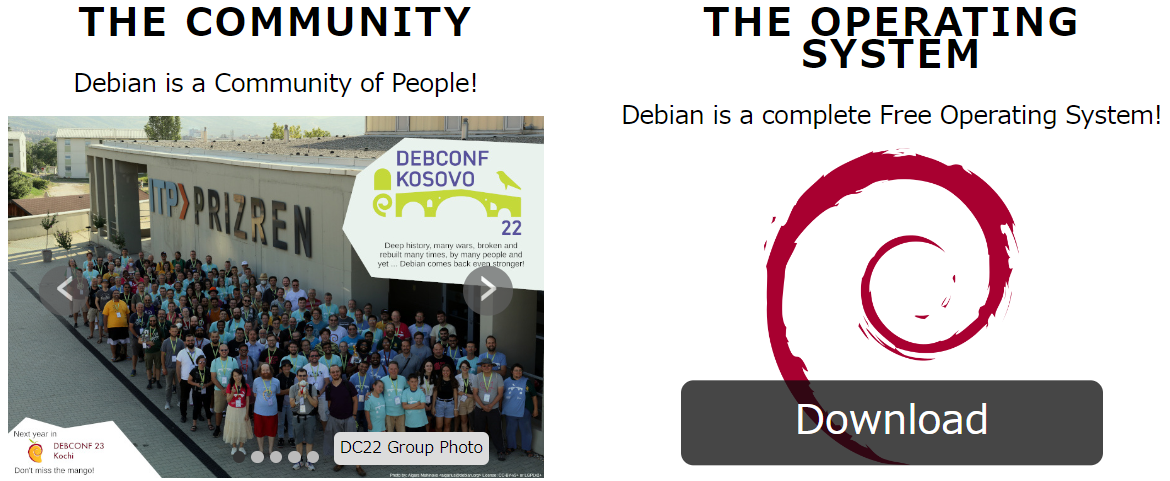
\includegraphics[scale=0.35]{image202303/www-debian-org-2022.png}
%{\small (画像出典:\url{https://www.debian.org/})}

\begin{itemize}
\item \url{https://www.debian.org/}
\item ボランティアで{\color{red}{フリー/オープン}}で{\color{red}{ユニバーサル}}な \\
「オペレーティングシステム (OS) 」を開発する\\
「コミュニティ」
\end{itemize}

\end{frame}


\subsection{Debian と OS}


\begin{frame}{Debian というオペレーティングシステム}

Debian はボランティアのみで開発しています

\begin{table}[htb]
  \begin{tabular}{|c|c|c|}
    \hline
    \textbf{ディストリ} & \textbf{企業}& \textbf{ボランティア} \\ \hline
    Fedora & Red Hat支援あり & あり  \\ \hline
    CentOS Stream & Red Hat支援あり & あり \\ \hline
    RHEL\footnote{Red Hat Enterprise Linux} & Red Hat & なし  \\ \hline
    \color{red}{Debian}  & \color{red}{なし} & \color{red}{あり} \\ \hline
    Ubuntu  & Canonical & あり \\ \hline
    openSUSE & SUSE支援あり & あり \\ \hline
    SLES\footnote{SUSE Linux Enterprise Server} & SUSE & なし \\ \hline
  \end{tabular}
\end{table}

\end{frame}

\begin{frame}{Debian というオペレーティングシステム}

\begin{itemize}
\item 様々な用途に使える汎用的な作り
  \begin{itemize}
  \item ノート PC、デスクトップ PC などの普段利用するコンピュータの OS
  \item Linux サーバ
    \begin{itemize}
    \item web サーバのシェア\footnote{\url{https://w3techs.com/technologies/details/os-linux/all/all}}:\\ Linuxサーバの内、Ubuntu 32.0 \%、Debian 16.7 \%、CentOS 8.4 \%
    \end{itemize}
  \item 組込デバイスのベース OS (多くの CPU で動作する)
  \end{itemize}
\item 「Debian」ベースな派生OSの源流
  \begin{itemize}
  \item 例:Ubuntu、Kali Linux、Raspberry Pi OS
    % https://debian-handbook.info/browse/en-US/stable/sect.ubuntu.html
    % https://debian-handbook.info/browse/en-US/stable/sect.kali.html
    % https://debian-handbook.info/browse/en-US/stable/sect.raspbian.html
  \item 派生先のディストリビューションと相互に情報交換をして開発している
  \end{itemize}
\end{itemize}

\end{frame}


\begin{frame}{Debian というオペレーティングシステム}
  \begin{itemize}
  % https://www.debian.org/News/2022/20221217
  \item 2023 年 3 月の時点で、最新の安定版は {\color{red}{Debian 11.6}}
    \begin{itemize}
    \item コードネーム: bullseye
    % https://www.debian.org/releases/bullseye/amd64/release-notes/ch-whats-new.ja.html
    \item パッケージ数は {\color{red}{約59,551}} 以上を提供
    \item 公式にサポートする CPU アーキテクチャは {\color{red}{9 つ}}
    \end{itemize}
  \item コードネームはトイ・ストーリーのキャラクター名を採用
  \item 次のメジャーリリース は Debian 12
    \begin{itemize}
    \item コードネーム: {\color{red}{bookworm}}
    \item 2023 年夏頃にリリースすると思われる
    \end{itemize}
\end{itemize}

\end{frame}


\begin{frame}{Debian というオペレーティングシステム}

リリースサイクル

\begin{itemize}
\item メジャーリリース:おおよそ 2 年ごと
  \begin{itemize}
  \item Debian は time-based freeze を採用
    % https://www.debian.org/News/2009/20090729
  \end{itemize}
\item 標準サポート:3年
  % https://www.debian.org/releases/
\item LTS\footnote{Long Term Support}:標準サポート終了後から 2 年
  \begin{itemize}
  % \item \url{https://wiki.debian.org/LTS}
  \item 対象アーキテクチャは amd64、i386、arm 系に限定
  \item 主要なパッケージのみサポート (全パッケージではない)
  %\item スポンサーとして資金援助するとメンテナンスするパッケージの希望を出せる
  \end{itemize}
\item Extended LTS:LTS 終了後から 5 年
  \begin{itemize}
  % \item \url{https://wiki.debian.org/LTS/Extended}
  \item 公式の Debian プロジェクトの運営ではなく、LTS をメンテナンスしている Freexian の商用サービス
  \item 契約者がサポートするパッケージを指定する
  \item 更新やセキュリティ修正したパッケージはすべての Debian ユーザーが無料で利用可能
  \item お願い:できるだけ次のバージョンに上げてください
  \end{itemize}
\end{itemize}

\end{frame}


\subsection{Debian と コミュニティ}


\begin{frame}{Debian というコミュニティ}

Debian への参加者は世界中にいます

\begin{itemize}
\item Debian 開発者 (Debian Developer、DD)
  \begin{itemize}
  \item Debian Project の公式開発者
  \item 57 ヶ国に 938 名 (2023-03-05 時点)\footnote{\url{https://people.debian.org/~eriberto/udd/dd-by-country.html}}
  \item 日本に在住している人は 34 人
  \item 国別人数ではドイツ、アメリカ、フランス、イギリスに次いで第 5 位
  \end{itemize}
\item Debian メンテナー (Debian Maintainer、DM)
\item パッケージメンテナー
\item ドキュメントなどの翻訳
\item そのほかにも多くの貢献者たちが Debian に参加
\end{itemize}
  
\end{frame}


\begin{frame}{Debian というコミュニティ}

\begin{itemize}
\item Debian 社会契約\footnote{\url{https://www.debian.org/social_contract}}
  \begin{itemize}
  \item Debian 開発者 たちが目指すフリーソフトウェアコミュニティの在り方
  \end{itemize}
\item Debian フリーソフトウェアガイドライン(DFSG)
  \begin{itemize}
  \item Debian 社会契約の一部
  \item Debian が考えるフリーソフトウェアの定義
  \item オープンソースの定義のひな形にもなっている
  \end{itemize}
\item Debian Policy\footnote{\url{https://www.debian.org/doc/debian-policy/}}
  \begin{itemize}
  \item Debian パッケージの区分、内容、ルール、ファイル配置の方針などの技術的な定義
  \end{itemize}
\end{itemize}

\end{frame}


\begin{frame}{Debian というコミュニティ}%[containsverbatim]

DebConf
  
\begin{itemize}
\item 年に一度、Debian 開発者が集まって開催するカンファレンス
\item 通常はオフラインで集まるが、COVID-19 の影響で 2020 年と 2021 年はオンラインで開催
  \begin{itemize}
  \item 2019/07/21 - 07/28: Debconf19: CURITIBA, BRAZIL
  \item 2020/08/23 - 08/29: Debconf20: Online
  \item 2021/08/24 - 08/28: Debconf21: Online
  \item 2022/07/17 - 07/24: Debconf22: Prizren, Kosovo
    \begin{itemize}
    \item \url{https://debconf22.debconf.org/}
    \item 発表のビデオがありますのでぜひご覧ください
    \end{itemize}
  \item 2023/09/10 - 09/17 (予定): Debconf23: Kochi, India
    \begin{itemize}
    \item \url{https://debconf23.debconf.org/}
    \end{itemize}
  \end{itemize}
\end{itemize}

%\begin{center}
  % https://wiki.debian.org/DebConf/22/Photos
%\end{center}

\end{frame}

\subsection{まとめ}

\begin{frame}{Debian とは?}
  
まとめると「Debian」とは

\begin{itemize}
  \item フリー/オープンな「オペレーティングシステム (OS) 」を作成しようとする人たちが集まるボランティアベースの「プロジェクト」
  \item 自分たちの考えるフリーという言葉に関する定義、開発目的、パッケージングポリシーを厳格に決めている
  \item 世界中に 900 人以上の公式開発者がおり、他のディストリビューションのベースとして採用されている
  \item 約 2 年毎にリリースが行われ、多くのパッケージとアーキテクチャをサポートしている
  \item 上記のような特徴から様々なところで利用されている Linux ディストリビューション
\end{itemize}

\end{frame}

%------------------


\section{Debian JP Project と Debian勉強会}


\begin{frame}
  \begin{center}\Huge{Debian JP Project\\と\\Debian勉強会}\end{center}
\end{frame}

\subsection{Debian JP Projectとは}
  
\begin{frame}{Debian JP Project とは?}

\begin{itemize}
  \item \url{https://www.debian.or.jp/}
  \item 日本において Debian を普及させることを目的とした任意団体
  \item 活動内容
  \begin{itemize}
    \item Debian の日本語による情報発信
    \item ユーザとの情報交換
    \item Debian 開発者やパッケージメンテナの育成など
  \end{itemize}
\end{itemize}

\end{frame}


\subsection{Debian勉強会}


\begin{frame}{Debian勉強会}

\begin{itemize}
 \item 2005 年 1月開始
 \item Debian 開発者 上川さんが発起人
 \item 東京と関西で月に一回コンスタントに開催しているDebian 開発者、Debian ユーザによる勉強会
   \begin{itemize}
   \item 東京エリアDebian勉強会
     \begin{itemize}
     \item \url{https://tokyodebian-team.pages.debian.net/}
     \end{itemize}
   \item 関西Debian勉強会
     \begin{itemize}
     \item \url{https://wiki.debian.org/KansaiDebianMeeting}
     \end{itemize}
   \item COVID-19 のため、2020 年 3 月からは東京エリアと関西でオンラインによる合同勉強会を開催中
   \end{itemize}
\end{itemize}

\end{frame}


\begin{frame}{Debian勉強会:解決したい内容}

\begin{itemize}
 \item 問題
   \begin{itemize}
   \item ML と IRC で情報交換していた
   \item face-to-face で会う場所がない
   \item まとまったドキュメントが出てこない
   \end{itemize}
 \item Debian 勉強会の提案
   \begin{itemize}
   \item 定期的に集まる
   \item 資料を作成して公開(GPL-2+) \\
	 {\small \url{https://salsa.debian.org/tokyodebian-team/monthly-report}}
   \end{itemize}
\end{itemize}

\end{frame}


\subsection{最近の勉強会}


\begin{frame}{Debian勉強会:最近の勉強会}
  
\begin{itemize}
\item 勉強会の内容
  \begin{itemize}
  \item Debian 界隈やパッケージング関連の話題など専門の人に話を聞く
  \item Debianで気になった事柄を調べてレポートする
  \end{itemize}
\item 前回の内容(2月):
  \begin{itemize}
  \item 場所: オンライン
  \item セミナー「DDTP及びDDTSSの紹介」
  \item ハンズオン「DDTSSを使ってパッケージ説明文を翻訳してみよう」
  \end{itemize}
\item 各地のイベントでDebian普及活動
  \begin{itemize}
  \item OSC2021東京
  %\item OSC2019北海道、OSC2019京都、OSC2019東京
  %\item 関西オープンフォーラム
  \end{itemize}
\end{itemize}

\end{frame}

%-----------------------

\section{次期安定版 Debian 12 bookworm}

\begin{frame}
  \begin{center}\Huge{Debian 12 bookworm}\end{center}
\end{frame}


\begin{frame}{Debian 12 bookworm}% [containsverbatim]

Debian 12 (コードネーム:bookworm)

\begin{itemize}
\item 現在開発を進めている次の安定版リリース
\item \url{https://wiki.debian.org/DebianBookworm}
\item Debian は time-based freeze を採用しており、およそ2年毎のリリースを目指す
\item サポートするアーキテクチャはまだ確定していない
  \begin{itemize}
  \item 参考:Debian 11 でサポートしているアーキテクチャ
    \begin{itemize}
    \item amd64, i386 (i686以降)
    \item arm64, armhf, armel
    \item mips64el, mipsel
    \item ppc64el
    \item s390x
    \end{itemize}
  \end{itemize}
\end{itemize}
  \begin{center}
    %\includegraphics[width=0.6\hsize]{image202303/bookworm.jpg}
    % https://pixar.fandom.com/wiki/Bookworm
  \end{center}
\end{frame}


\subsection{インストーラ}


\begin{frame}{Debian 12 bookworm}% [containsverbatim]

Debian Installer Bookworm Alpha 2 release

\begin{itemize}
  \item \url{https://www.debian.org/devel/debian-installer/News/2023/20230219}
  \item いち早く bookworm を試してみたい方は以下からダウンロードしてインストールできます
    \begin{itemize}
    \item \url{https://www.debian.org/devel/debian-installer/index.ja.html}
    \item 自分の環境でインストールがうまく行われない場合はインストールレポートをお願いします
    \item \url{https://www.debian.org/releases/bookworm/amd64/apas04.ja.html} 
  \end{itemize}
\end{itemize}

\end{frame}


\subsection{テーマ}


\begin{frame}{Debian 12 bookworm}% [containsverbatim]

テーマ

\begin{itemize}
\item 次期安定版に採用するテーマは通常コンテストを行う
\item しかし、今回は応募が 3 つと少なかったためコンテストは行わなかった
\item Juliette Taka さん提供の「Emerald」で異論が出なければ、これが採用予定
\item \url{https://wiki.debian.org/DebianArt/Themes/Emerald}
\end{itemize}

\begin{center}
  
\includegraphics[width=0.60\hsize]{image202303/Emerald-wallpaper_1920x1080.png}
\end{center}

\end{frame}


\subsection{提供ソフトウェアのバージョン}


\begin{frame}{Debian 12 bookworm}% [containsverbatim]

ソフトウェアは以下のバージョンでテスト中

\begin{itemize}
\item Linux カーネル 6.1
\item ツールチェイン GCC 10.4.0, binutils 2.40, glibc 2.36, LLVM 14.0.6, 13.0.1
\item Perl 5.36.0, Python 3.11.2, Ruby 3.1.2, PHP 8.2.2, Go 1.19.6, OpenJDK 17.0.6
\item GNOME 43, KDE Plasma 5.27.0, Cinnamon 5.6.7, MATE 1.26, Xfce 4.18, lxde 0.99.2, lxqt 1.2.0
\item MariaDB 10.11.2, PostgreSQL 15.2, sqlite 3.40.1 
\item OpenSSH 9.2p1, OpenSSL 3.0.8, GnuPG 2.2.40/1.4.23
\item etc..
\end{itemize}

\end{frame}


\subsection{リリースまでの流れ}

\begin{frame}{Debian 12 bookworm}% [containsverbatim]

Debian 12 はいつリリースされるのか?

\begin{itemize}
\item Debianのリリース条件は「リリースクリティカルバグ(RC bug)が 0 個になったとき」
\item 2023-03-06 現在のリリースクリティカルバグの一覧
  \begin{itemize}
  \item \url{https://bugs.debian.org/release-critical/}
  \end{itemize}
\end{itemize}

\begin{center}
  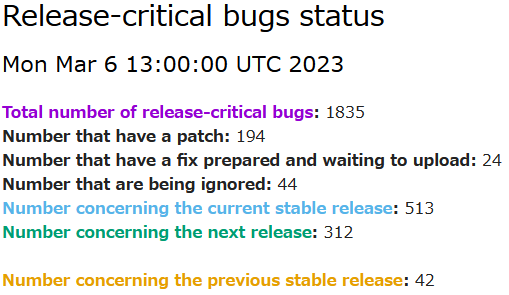
\includegraphics[width=0.45\hsize]{image202303/debian-rcbug-1_20230306.png}
  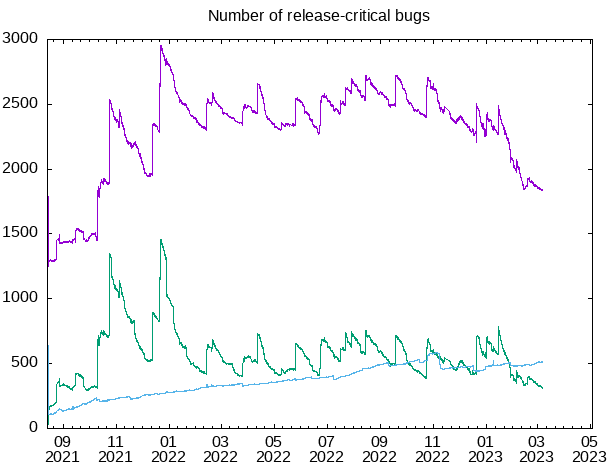
\includegraphics[width=0.45\hsize]{image202303/debian-rcbug-2_20230306.png}
  % https://bugs.debian.org/release-critical/
\end{center}

\end{frame}


\begin{frame}{Debian 12 bookworm}% [containsverbatim]

リリースまでの流れ (フリーズスケジュール)\footnote{\url{https://release.debian.org/bookworm/freeze_policy.html}}

\begin{itemize}
\item 2023-01-12: Transition and Toolchain Freeze
  \begin{itemize}
  \item コンパイラ等のビルドツールやプログラム実行環境などの重要なパッケージのバージョンアップはここまで
  \end{itemize}
\item 2023-02-12: Soft freeze ←今はこの段階に入った状態
  \begin{itemize}
  \item この期日までに testing に移行しているパッケージが次の安定版リリースに含まれる
  \item この期日以降のパッケージの変更は小規模で的を絞った内容に限って行う
  \end{itemize}
\item 2023-03-12: Hard freeze
  \begin{itemize}
  \item 重要なパッケージや autopkgtests がないパッケージは unblock リクエスト\footnote{debdiff を添えて unblock というバグ報告を行い、リリースチームのレビューを受ける必要あり} が必要
  \end{itemize}
\item 未定: Full freeze
  \begin{itemize}
  \item すべてのパッケージにおいて unblock リクエストが必要
  \end{itemize}
\end{itemize}
\end{frame}


\subsection{Debian 12 の変更点}

\begin{frame}
  \begin{center}\Huge{Debian 12 の変更点}\end{center}
\end{frame}


\begin{frame}{Debian 12 の変更点}% [containsverbatim]

【ご注意ください】

まだリリースノートは出ていません。今後変わることがあります。

\end{frame}

% aptのnon-free-firmwareセクションの導入
%% debian installerも変更
% usrmerge
% python の pip のbroken
% python2 が完全除去された

% from apt-listchanges
%
% adduser
% anacron
% apache2
% fonts-urw-base35
% glibc
% isc-dhcp-client
% libraw
% libtirpc
% scowl
% shadow
% systemd
% grep
% apt
% gdm3
% modemmanager
% openssh
% policykit-1
% procps
% libreoffice

\begin{frame}[containsverbatim]{Debian 12 の変更点}

apt に non-free-firmware セクションが追加 \\
Debian Installer は non-free な firmware を含めた形で提供

\begin{commandlinesmall}
- debian 11
  deb http://deb.debian.org/debian/ bullseye main
- debian 12
  deb http://deb.debian.org/debian/ bookworm main non-free-firmware
\end{commandlinesmall}

\begin{itemize}
\item Debian では「Debian 社会契約」でフリーと定めたパッケージのみインストーラに含めてきた
\item 無線 LAN や GPU のドライバ等の動作には non-free なファームウェアが必要で、インストール時に ハードウェアが認識しないため不便という声がある
\item Debian 開発者による投票で「Debian 社会契約」を変更して実現\footnote{\url{https://www.debian.org/vote/2022/vote_003}}
\end{itemize}

\end{frame}


\begin{frame}{Debian 12 の変更点}% [containsverbatim]

/usr merge が適用された

\begin{itemize}
\item \url{https://wiki.debian.org/UsrMerge}
\item /bin、/sbin、/lib 系のディレクトリは /usr配下へのシンボリックリンク
\item /bin → usr/bin、/sbin → usr/sbin
\item /lib → usr/lib
\item /lib64 → usr/lib64、/lib32 → usr/lib32、\\ /libx32 → usr/libx32 
\end{itemize}

\end{frame}


\subsection{バグレポート}

\begin{frame}{バグレポートをお願いします}% [containsverbatim]
  \begin{itemize}
  \item 何かおかしい動作や不具合を見つけた場合はバグレポートをお願いします
  \item バグレポートの仕方(レポートは英語で送る必要あり)
    \begin{itemize}
    \item \url{https://www.debian.org/Bugs/Reporting.ja.html}
    \end{itemize}
  \item バグレポートの前にちょっと相談してみたい方は、日本語のDebian JPメーリングリストや、SNSで相談してみてください
    \begin{itemize}
    \item \url{https://www.debian.or.jp/community/ml/openml.html}
    \item Twitter: @debian\_jp
    \end{itemize}
  \end{itemize}
\end{frame}

%-----------------------

%\section{Debian Updates}

% 半年間の以下MLから抜粋して紹介する
%  debian-announce@lists.debian.org
%  debian-devel-announce@lists.debian.org

%\begin{frame}
%  \begin{center}\Huge{Debian Updates}\end{center}
%\end{frame}


%\subsection{released timeline}

%\begin{frame}{Debian Updates}% [containsverbatim]

%\begin{itemize}
%\item 2021/02/06:  Updated Debian 10.8  released
%\item 2021/03/27:  Updated Debian 10.9  released
%\item 2021/06/19:  Updated Debian 10.10 released
%\item 2021/08/14:  Debian 11 released
%\item 2021/10/09:  Updated Debian 10.11 released
%\item 2021/10/09:  Updated Debian 11.1  released
%\end{itemize}

%\end{frame}


%\subsection{Bits from the DPL}

%\begin{frame}{Debian Updates}% [containsverbatim]

%Bits from the DPL

%\begin{itemize}
%\item 月に一度の Debian Project Leader である jcc さんのプロジェクトの進捗を報告
%\item 時間のない方でもこれを読んでおけば Debian Project の大まかな動きがわかる
%\end{itemize}

%\small{
%\begin{itemize}

%\item 2021/08/30 \url{https://lists.debian.org/debian-devel-announce/2021/08/msg00005.html}

%\end{itemize}
%}

%\end{frame}


%-----------------------

\section{日本語によるDebianの情報}

\begin{frame}\begin{center}\Huge{日本語によるDebianの情報}\end{center}\end{frame}

\begin{frame}{日本語によるDebianの情報}
\begin{itemize}
  \item Debian JP Project \\
      \url{https://www.debian.or.jp}
  \item 東京エリアDebian勉強会\\
      \url{https://tokyodebian-team.pages.debian.net/}
  \item 関西Debian勉強会 \\
      \url{https://wiki.debian.org/KansaiDebianMeeting}
  \item Twitter \\
      \url{@debian_jp}
\end{itemize}
\end{frame}

%----------------

\section{今後のイベント}

\begin{frame}\begin{center}\Huge{今後のイベント}\end{center}\end{frame}


\begin{frame}{今後のイベント}

\begin{itemize}
\item 4/1(土) OSC 2023 Tokyo/Spring
  \begin{itemize}
  \item \url{https://event.ospn.jp/osc2023-spring/}
  \item ブース出展します
  \end{itemize}
\item 4/15(土) 東京エリア・関西合同 Debian 勉強会(オンライン開催)
  \begin{itemize}
  \item \url{https://tokyodebian-team.pages.debian.net/2023-04.html}
  \item 発表者を募集中
  \end{itemize}
\end{itemize}

\end{frame}

%----------------

\end{document}

;;; Local Variables: ***
;;; outline-regexp: "\\([ 	]*\\\\\\(documentstyle\\|documentclass\\|emtext\\|section\\|begin{frame}\\)\\*?[ 	]*[[{]\\|[]+\\)" ***
;;; End: ***
